\documentclass[a4]{article}
\usepackage{geometry}
\geometry{verbose,tmargin=2.5cm,bmargin=2.5cm,lmargin=3cm,rmargin=3cm}
\usepackage{amsmath,amssymb,amsthm}
\usepackage{graphicx}
\graphicspath{{graphics/}}
\usepackage[utf8]{inputenc}
\usepackage{fancyvrb}
\usepackage{hyperref}
\usepackage{lscape}
\usepackage{adjustbox}
\usepackage{verbatim}
\usepackage{subcaption}
\usepackage{placeins}
\usepackage{array}
\usepackage{multirow}
\usepackage{makecell}

\title{MultiFEBE \\ Tutorial 8: impedances of a suction caisson}
\author{\'A.G. Vega-Artiles}
\date{May 2023}

\begin{document}

\maketitle

\tableofcontents

\section{Problem description}

In this eighth tutorial, the impedances of a suction caisson are obtained. Figure \ref{fig:geometry_suction_caisson} shows the geometry. 

\begin{figure}[tbh!]
	\centering
	\includegraphics[scale=0.6]{geometry_suction_caisson.png}
	\caption{Geometry of the suction caisson.}
	\label{fig:geometry_suction_caisson}
\end{figure}

Required material and geometric properties are the Young's modulus $E$, the Poisson's ratio $\nu$, the density $\rho$, the hysteretic damping $\xi$, the skirt length and thickness $L$ and $t$ and the lid diameter $D$. Self-weight is not considered.

The following equations will be used: 

\begin{equation}
	\begin{array}{l}
		a_0 = \omega R/c_{soil} \medspace \mathrm{(dimensionless)} \\
		c_{soil} = \sqrt{\mu_{soil}/\rho_{soil}}\medspace \mathrm{(m/s)} 
	\end{array}
\end{equation}

The problem is solved for $L=10$ $\mathrm{m}$, $D=10$ $\mathrm{m}$,  $t=0.05$ $\mathrm{m}$, $E_{sc} = 210 \cdot 10^9$ $\mathrm{N/m^2}$, $\nu_{sc}=0.25$, $\nu_{soil}=0.33$, $\rho_{sc}=10^{-6}$ $\mathrm{kg/m^3}$, $\rho_{soil}=1000$ $\mathrm{kg/m^3}$, $\mu_{soil}=10^{6}$ $\mathrm{N/m^2}$, $\xi_{sc}=0.01$, $\xi_{soil}=0.025$.

\begin{equation}
	\begin{array}{l}
		c_{soil} = 31.62 \medspace \mathrm{m/s} \\
		a_0 = 0.01 \medspace \Longrightarrow \omega = 0.063 \medspace \mathrm{rad/s}\\
		a_0 = 10 \medspace \Longrightarrow \omega = 63.246 \medspace \mathrm{rad/s}
	\end{array}
\end{equation}

\section{Pre-processing} 
Pre-processing in MultiFEBE consists of defining the geometry and mesh of the problem. There are three ways to do such definition: directly from the input file (mode = 0), from another file in the native format (mode = 1) or from another file in the Gmsh MSH file format version 2.2 (mode = 2). However, it is preferable to use a *.msh file for relatively large geometries, therefore, this is the syntax explained in the following subsections.
   
\subsection{Mesh generation with Gmsh}
Gmsh \cite{gmsh, gmshweb} is a finite element mesh generator with its own language. The software allows to create the geometry in a “bottom-up” manner, going from the most basic elements (points) to the highest order elements (volumes) or in a “Constructive Solid Geometry” manner (boolean operations) or with a combination of methodologies. Gmsh also allows to define  the so-called “physical groups” which are unmodifiable entities that gather elementary entities as sole entities, where every entity must have a unique tag. On the other hand, the file containing all this geometric definition is the *.geo file whereas the mesh definition is in the *.msh file. 

\subsubsection{GEO file}
The Gmsh language allows to define parameters to use later in the script and comments as every other programming language. 

In this example several parameters are defined: diameter (D), length (L), the mesh element size for the suction caisson and the free surface near it (ms\_near), the mesh element size far from the suction caisson (ms\_far) and the radius of the free surface (R\_truncation). 

<<<<<<< HEAD
Every point in the geometry can be specified by its coordinates (x y z) and mesh element size with the function ``Point". Every straight line of the model is created with the function ``Line" and its initial and final points. Then, with the function ``Physical Line" every line is converted into a single entity or physical entity with its own name. Furthermore, the function ``Transfinite Line" explicitly defines the location of the nodes on the line by following the expression specified and the function ``Round" rounds values to the nearest integer. Every ruled surface is created with the function ``Ruled Surface" by setting its perimeter with the function ``Line Loop" and the lines used to close the surface. The function ``Transfinite surface" meshes surfaces with the 2D transfinite algorithm and ``Recombine Surface" transforms meshes into mixed triangular/quadrangular meshes. Moreover, with the function ``Physical Surface" every surface is converted into a single entity or physical entity with its own name.  
=======
Every point in the geometry can be specified by its coordinates (x y z) and mesh element size with the function "Point". Every straight line of the model is created with the function "Line" and its initial and final points. Then, with the function "Physical Line" every line is converted into a single entity or physical entity with its own name. Furthermore, the function "Transfinite Line" explicitly defines the location of the nodes on the line by following the expression specified and the function "Round" rounds values to the nearest integer. Every ruled surface is created with the function "Ruled Surface" by setting its perimeter with the function "Line Loop" and the lines used to close the surface. The function "Transfinite surface" meshes surfaces with the 2D transfinite algorithm and "Recombine Surface" transforms meshes into mixed triangular/quadrangular meshes. Moreover, with the function "Physical Surface" every surface is converted into a single entity or physical entity with its own name.  
>>>>>>> main

It is worth noting that “if an expression defines a new entity, it is enclosed between parentheses but if an expression refers to a previously defined entity, it is enclosed between braces.” \cite{gmshweb}

The resulting *.geo file applied to the problem is the following:

\begin{Verbatim}
// Geometry & mesh parameters
D = 10;
L = 10;
ms_near = 1;
ms_far = 2;
R_truncation = 3*D;

/*
bucket-skirt
*/
Point (1) = { D/2 ,   0 ,  0 , ms_near };
Point (2) = {   0 ,   0 ,  0 , ms_near };
Point (3) = {   0 , D/2 ,  0 , ms_near };
Point (4) = {   0 , D/2 , -L , ms_near };
Point (5) = {   0 ,   0 , -L , ms_near };
Point (6) = { D/2 ,   0 , -L , ms_near };
Circle (1) = {1,2,3};
Line (2) = {3,4}; 
Circle (3) = {4,5,6};
Line (4) = {6,1};
Line Loop (5) = {1,2,3,4};
Transfinite Line{1,3}=Round(0.25*Pi*D/ms_near+1.);
Transfinite Line{2,4}=Round(L/ms_near+1.);
Ruled Surface (1) = {5};
Transfinite Surface {1};
Recombine Surface{1};
Color {196,196,196} { Surface {1};}

/*
soil-skirt
*/
Point (11) = { D/2 ,   0 ,  0 , ms_near };
Point (12) = {   0 ,   0 ,  0 , ms_near };
Point (13) = {   0 , D/2 ,  0 , ms_near };
Point (14) = {   0 , D/2 , -L , ms_near };
Point (15) = {   0 ,   0 , -L , ms_near };
Point (16) = { D/2 ,   0 , -L , ms_near };
Circle (11) = {11,12,13};
Line (12) = {13,14}; 
Circle (13) = {14,15,16};
Line (14) = {16,11};
Line Loop (15) = {11,12,13,14};
Transfinite Line{11,13}=Round(0.25*Pi*D/ms_near+1.);
Transfinite Line{12,14}=Round(L/ms_near+1.);
Ruled Surface (11) = {15};
Transfinite Surface {11};
Recombine Surface{11};
Color {196,98,0} { Surface {11};}

/*
Pile top
*/
Point (17) = {   0 ,   0 , 0 , ms_near };
Point (18) = { D/2 ,   0 , 0 , ms_near };
Point (19) = {   0 , D/2 , 0 , ms_near };
Circle(17) = {18,17,19};
Line  (18) = {19,17};
Line  (19) = {17,18};
Transfinite Line{17}=Round(0.25*Pi*D/ms_near+1.);
Line Loop (20) = {17,18,19};
Plane Surface(17) = {20};
Color {128,64,0} { Surface {17};}

/*
Free-surface
*/
Point (31) = {   0 ,   0 , 0 , ms_near };
Point (32) = { D/2 ,   0 , 0 , ms_near };
Point (33) = {   0 , D/2 , 0 , ms_near };
Point (34) = { R_truncation ,           0. , 0. , ms_far };
Point (35) = {           0. , R_truncation , 0. , ms_far };
Circle(31) = {32,31,33};
Transfinite Line{31}=Round(0.25*Pi*D/ms_near+1.);
Circle(32) = {34,31,35};
Line  (33) = {32,34};
Line  (34) = {35,33};
Line Loop (35) = {33,32,34,-31}; 
Plane Surface(31) = {35};
Color {255,128,0} { Surface {31};}

/* Final order of Physical Surfaces */
Physical Surface("free-surface") = {31};
Physical Surface("bucket-lid") = {17};
Physical Surface("soil-skirt") = {11};
Physical Surface("bucket-skirt") = {1};

// Mesh generation
Mesh 2;
SetOrder 2;
Save "mesh.msh";
\end{Verbatim}

\begin{figure}[tbh!]
	\centering
	\includegraphics[scale=0.6]{geometry_geo.png}
	\caption{Geometry of the suction caisson from the *.geo file.}
	\label{fig:geometry_geo}
\end{figure}

\subsubsection{MSH file}

The *.msh file begins with a mandatory section about information of the file (MeshFormat) and following by the other sections. Here, three sections are used: the physical group names (PhysicalName), the nodes (Nodes) and the elements (Elements).

<<<<<<< HEAD
In the section ``PhysicalName", all the physical entities of the model are defined. The first line indicates the number of physical entities. Then, one line per physical entity indicating the physical dimension, the tag and the name.  

In the section ``Nodes", all the nodes of the model are defined. The first line indicates the number of nodes. Then, one line per node indicating the identifier of the node and its coordinates (x y z).

In the section ``Elements", all the elements of the model are defined. The first line indicates the number of elements. Then, one line per element indicating:
=======
In the section "PhysicalName", all the physical entities of the model are defined. The first line indicates the number of physical entities. Then, one line per physical entity indicating the physical dimension, the tag and the name.  

In the section "Nodes", all the nodes of the model are defined. The first line indicates the number of nodes. Then, one line per node indicating the identifier of the node and its coordinates (x y z).

In the section "Elements", all the elements of the model are defined. The first line indicates the number of elements. Then, one line per element indicating:
>>>>>>> main

\begin{itemize}
	\item Element identifier.
	\item Type of element.
	\item Number of auxiliary tags.
<<<<<<< HEAD
	\item List of tags, where the two first auxiliary tags are mandatory, and the first one corresponds to the identifier of the physical entity to which the element belongs and the second one is the identifier of the elementary model entity to which the element belongs. The rest of the tags are optional.
=======
	\item List of tags, where the two first auxiliary tags are mandatory, and corresponds to the identifier of the physical entity to which the element belongs and the second one is the identifier of the elementary model entity to which the element belongs. The rest of the tags are optional.
>>>>>>> main
	\item A list of identifiers corresponding to the nodes of the element.
\end{itemize}

For example, in this case, an element with the identifiers 1 9 2 2 17 10 152 895 159 906 907 corresponds to:

\begin{itemize}
	\item 1: element 1.
	\item 9: type 9 (9-node second order quadrangle).
	\item 2: it has 2 auxiliary tags.
	\item 2: it belongs to the physical entity 2.
	\item 17: it belongs to the surface 17.
	\item 10, 152, 895, 159, 906, 907: it connects the nodes 10, 152, 895, 159, 906 and 907.
\end{itemize} 

\begin{figure}[tbh!]
	\centering
	\includegraphics[scale=0.6]{mesh.png}
	\caption{Mesh of the suction caisson from the *.msh file.}
	\label{fig:mesh}
\end{figure}

\subsection{Input data file}
Solving in MultiFEBE consists of running the software by specifying several options in the following sections\footnote{See reference manual.}: [problem], [settings], [materials], [regions], [conditions over nodes], etc.

The first part to configurate is the problem definition in the section [problem]. This example is a 3D harmonic mechanical problem.

\begin{Verbatim}	
[problem]
n = 3D
type = mechanics
analysis = harmonic
\end{Verbatim}

Then, a list of frequencies is generated by specifying the number of frequencies, that must be $\geq 2$, (100), followed by the minimum frequency, $>$ 0, (0.063) and the maximum frequency (63.246), being each one in new lines.

\begin{Verbatim}
[frequencies]
rad/s
lin
100
0.063
63.246
\end{Verbatim}

<<<<<<< HEAD
In the section [export], several export and notation settings are defined. In this example, the nodal solutions and the stress resultant solutions will be exported by writing the option F or T with the corresponding expression, ``export\_nso" and ``export\_tot", respectively. Furthermore, the complex notation is set as cartesian. 
=======
In the section [export], several export and notation settings are defined. In this example, the nodal solutions and the stress resultant solutions will be exported by writing the option F or T with the corresponding expression, "export\_nso" and "export\_tot", respectively. Furthermore, the complex notation is set as cartesian. 
>>>>>>> main

\begin{Verbatim}
[export]
export_nso = T
export_tot = T
complex_notation = cartesian
\end{Verbatim}

Next step is to configurate the mesh. In this case, a mesh from Gmsh will be used so that it is necessary to write the option number 2 and the document name obtained from it in the section [settings]. However, if the mesh were going to be read from the input file, it would require to write the sections [nodes], [elements] and [parts] instead.

\begin{Verbatim}	
[settings]
mesh_file_mode = 2 "mesh.msh"
\end{Verbatim}

As the problem has two materials, the section [materials] will need three lines: a first line for the number of materials in the model and a line per material with its properties such as tag, type, $\rho$, E, $\nu$, $\mu$ and $ \xi $.

\begin{Verbatim}
[materials]
2
1 elastic_solid rho 1000. mu 1.E6 nu 0.33 xi 0.025
2 elastic_solid rho 1.E-6 E 210.E9 nu 0.25 xi 0.01
\end{Verbatim}

In the section [boundaries], all boundaries are defined. The first line indicates the number of boundaries (2). Then, one line per boundary indicating the boundary identifier, the part identifier that discretizes it, and finally the boundary class (ordinary).

\begin{Verbatim}
[boundaries]
2
1 1 ordinary
2 2 ordinary
\end{Verbatim}

In the section [be body loads], all body loads in BE regions are defined. The format consists of a first line with the number of BE body loads to be defined (1), next as many lines as BE body loads. Each line contains first the BE body load identifier (1) and last the mesh part which contains the elements associated with it (3).

\begin{Verbatim}
[be body loads]
1
1 3
\end{Verbatim}

The section [fe subregions] indicates the number of fe subregions in the first line (1) and a line per subregions indicating the subregion identifier (1) and the part identifier (4). The last two zeros at the end are mandatory and they are going to be used in the future for additional features.

\begin{Verbatim}
[fe subregions]
1
1 4 0 0
\end{Verbatim}

In the section [cross sections], it is necessary to specify the number of cross sections in the first line (1) and a line per cross section by indicating the type of fe (shell), number of fe subregions related to the cross section (1), fe subregion identifier (1) and the section thickness (0.05).

\begin{Verbatim}
[cross sections]
1
shell 1 1 0.05
\end{Verbatim}

The format of the section [regions] consists of a first line indicating the number of regions (2). Furthermore, for each region there must be a block of data consisting of several lines. 

<<<<<<< HEAD
The first region is a BE region, so the first line shows the region identifier and the region class (discretization method) (1 be). The second line indicates the number and list of boundaries (2 1 2), the third line defines the material (material 1), the fourth line defines the number and list of BE body loads (1 1) and the fifth line the number and list of incident fields (0).
=======
The first region is a BE region, so the first line shows the region identifier and the region class (discretization method) (1 be). The second line indicates the number of boundaries and a list of boundaries (2 1 2), the third line defines the material (material 1), the fourth line defines the number and a list of BE body loads (1 1) and the fifth line the number and a list of incident fields (0).
>>>>>>> main

The second region is a FE region, so the first line shows the region identifier and the region class (discretization method) (2 fe). Then, the second line indicates the number of subregions (1) and their identifiers (1) and the third line the material (material 2). 

\begin{Verbatim}	
[regions]
2

1 be
2 1 2
material 1 
1 1
0

2 fe
1 1
material 2 
\end{Verbatim}

In the section [groups], nodes and elements can be tagged depending on their position in space. The first line indicates the number of groups and then a line per group with the group tag and the command. In this example, a box is defined in space to select all the nodes inside it (nodes box interior) with its maximum and minimum x, y and z coordinates (-1.e3 1.e3 -1.e3 1.e3 -0.001 0.001), respectively, and the part where the nodes belong (4).    

\begin{Verbatim}
[groups]
1
1 nodes box interior -1.e3 1.e3 -1.e3 1.e3 -0.001 0.001 4 
\end{Verbatim}

In the section [fem node options], several options for the FE formulation can be set. In this example, the nodes belonging to group 1 are forced to have 6 degrees of freedom.  

\begin{Verbatim}
[fem node options]
group 1 n_dof 6
\end{Verbatim}

In the section [symmetry planes], all symmetry planes are defined assumed to be at the origin of coordinates. In order to indicate the existence and the nature of the symmetry, it is necessary to define up to three of the symmetry planes implemented: plane with unit normal $ \textbf{n} = \textbf{e}_1 = (1, 0, 0) $ (plane yz), plane with unit normal $ \textbf{n} = \textbf{e}_2 = (0, 1, 0) $ (plane zx), or plane with unit normal $ \textbf{n} = \textbf{e}_3 = (0, 0, 1) $ (plane xy); where each of one can be either of symmetry or antisymmetry

\begin{Verbatim}
[symmetry planes]
plane_n1: symmetry
plane_n2: antisymmetry
\end{Verbatim}

In the section [conditions over be boundaries], all boundaries will be specify in global coordinates because they are planar and their normal vectors are parallel to one of the global axes. As a 3D problem, there are three lines for every boundary: a first line for the x direction, the second one for the y direction and the third one for the z. In this example, an infinitesimal rotation field for the rocking impedance is used, so that the first number of every line indicates the type of condition (4), then the coordinates of the center of rotation (0., 0., 0.), the axis of rotation (0., 1., 0.) and the angle of rotation in complex number because it is a harmonic analysis.

\begin{Verbatim}
[conditions over be boundaries]
boundary 2: 4 0. 0. 0. 0. 1. 0. (1.,0.)
            4 0. 0. 0. 0. 1. 0. (1.,0.)
            4 0. 0. 0. 0. 1. 0. (1.,0.)
\end{Verbatim}

In the section [conditions over nodes], all boundary conditions over nodes or groups will be specified. As a 3D model, there are 6 lines for every boundary condition. In case of displacement, firstly the displacements $u_x, u_y, u_z$ are configured and then the rotations $\theta_x, \theta_y, \theta_z$. In case of force, firstly the forces $F_x, F_y, F_z$ and then the moments $M_x, M_y, M_z$. In this example, an infinitesimal rotation field for the rocking impedance is used, so that the first number of the three firsts lines indicates the type of condition (4), then the coordinates of the center of rotation (0., 0., 0.), the axis of rotation (0., 1., 0.) and the angle of rotation in complex number because it is a harmonic analysis. For the three last lines the rotations are configured with two digits, where the
first one indicates the type of condition (0 for displacement and 1 for force) and the second one the value in complex number.

\begin{Verbatim}	
[conditions over nodes]
group 1: 4 0. 0. 0. 0. 1. 0. (1.,0.)
         4 0. 0. 0. 0. 1. 0. (1.,0.)
         4 0. 0. 0. 0. 1. 0. (1.,0.)
         0 (0.,0.)
         0 (1.,0.)
         0 (0.,0.)
\end{Verbatim}

The whole data file applied to the problem is the following:

\begin{Verbatim}
[problem]
n = 3D
type = mechanics
analysis = harmonic

[frequencies]
rad/s
lin
100
0.063
63.246

[export]
export_nso = T
export_tot = T
complex_notation = cartesian

[settings]
mesh_file_mode = 2 "mesh.msh"

[materials]
2
1 elastic_solid rho 1000. mu 1.E6 nu 0.33 xi 0.025
2 elastic_solid rho 0. E 210.E9 nu 0.25 xi 0.01

[boundaries]
2
1 1 ordinary
2 2 ordinary

[be body loads]
1
1 3

[fe subregions]
1
1 4 0 0

[cross sections]
1
shell 1 1 0.05

[regions]
2
1 be
2 1 2
material 1 
1 1
0

2 fe
1 1
material 2 

[groups]
1
1 nodes box interior -1.e3 1.e3 -1.e3 1.e3 -0.001 0.001 4 

[fem node options]
group 1 n_dof 6

[symmetry planes]
plane_n1: symmetry
plane_n2: antisymmetry

[conditions over be boundaries]
boundary 2: 4 0. 0. 0. 0. 1. 0. (1.,0.)
            4 0. 0. 0. 0. 1. 0. (1.,0.)
            4 0. 0. 0. 0. 1. 0. (1.,0.)

[conditions over nodes]
group 1: 4 0. 0. 0. 0. 1. 0. (1.,0.)
         4 0. 0. 0. 0. 1. 0. (1.,0.)
         4 0. 0. 0. 0. 1. 0. (1.,0.)
         0 (0.,0.)
         0 (1.,0.)
         0 (0.,0.)
\end{Verbatim}

\section{Conditions for the impedance calculation}

The different conditions used for the calculation of all the impedances are shown in Table \ref{tab:conditions}. 

\begin{table}[h]
\centering
\caption{Conditions for the impedance calculation.}
\label{tab:conditions}
\begin{tabular}{|c|c c|c c|}
	\hline
	&  \multicolumn{2}{c|}{[conditions over boundaries]} & \multicolumn{2}{c|}{[conditions over nodes]}  \\
	\hline
	$ S_{HH} $ & boundary 2: & \makecell[c]{0 (1.,0.)\\
		0 (0.,0.)\\
		0 (0.,0.)} & group 1: & \makecell[c]{0 (1.,0.)\\
		0 (0.,0.)\\
		0 (0.,0.)\\
		0 (0.,0.)\\
		0 (0.,0.)\\
		0 (0.,0.)}\\
	\hline
	$ S_{VV} $ & boundary 2: & \makecell[c]{0 (0.,0.)\\
		0 (0.,0.)\\
		0 (1.,0.)} & group 1: & \makecell[c]{0 (0.,0.)\\
		0 (0.,0.)\\
		0 (1.,0.)\\
		0 (0.,0.)\\
		0 (0.,0.)\\
		0 (0.,0.)}\\
	\hline
	$ S_{MM} $ & boundary 2: & \makecell[c]{4 0. 0. 0. 0. 1. 0. (1.,0.)\\
	                                   4 0. 0. 0. 0. 1. 0. (1.,0.)\\
	                                   4 0. 0. 0. 0. 1. 0. (1.,0.)} & group 1: & \makecell[l]{4 0. 0. 0. 0. 1. 0. (1.,0.)\\
	                                                 4 0. 0. 0. 0. 1. 0. (1.,0.)\\
	                                                 4 0. 0. 0. 0. 1. 0. (1.,0.)\\
	                                                 0 (0.,0.)\\
                                                   	 0 (1.,0.)\\
	                                                 0 (0.,0.)} \\
	\hline
\end{tabular}
\end{table}

\section{Results and discussion}

Figure \ref{fig:results} shows the horizontal, vertical and rocking impedances for a suction caisson. The results from \cite{liingaard} are shown together with the results from the present approach. It is observed a very good agreement with respect to Liingaard \textit{et al.}. 

<<<<<<< HEAD
These results were obtained from the *.tot files by summing up the contributions of the ``bucket-lid" and the ``soil-skirt" for the target resultant forces or moments. For more details about the postprocessing see file ``tutorial\_008.m".
=======
These results were obtained from the *.tot files by summing up the contributions of the "bucket-lid" and the "soil-skirt" for the target resultant forces or moments. For more details about the postprocessing see file "tutorial\_008.m".
>>>>>>> main

\begin{figure}[tbh!]
	\centering
	\begin{subfigure}[b]{0.48\textwidth}
		\centering
		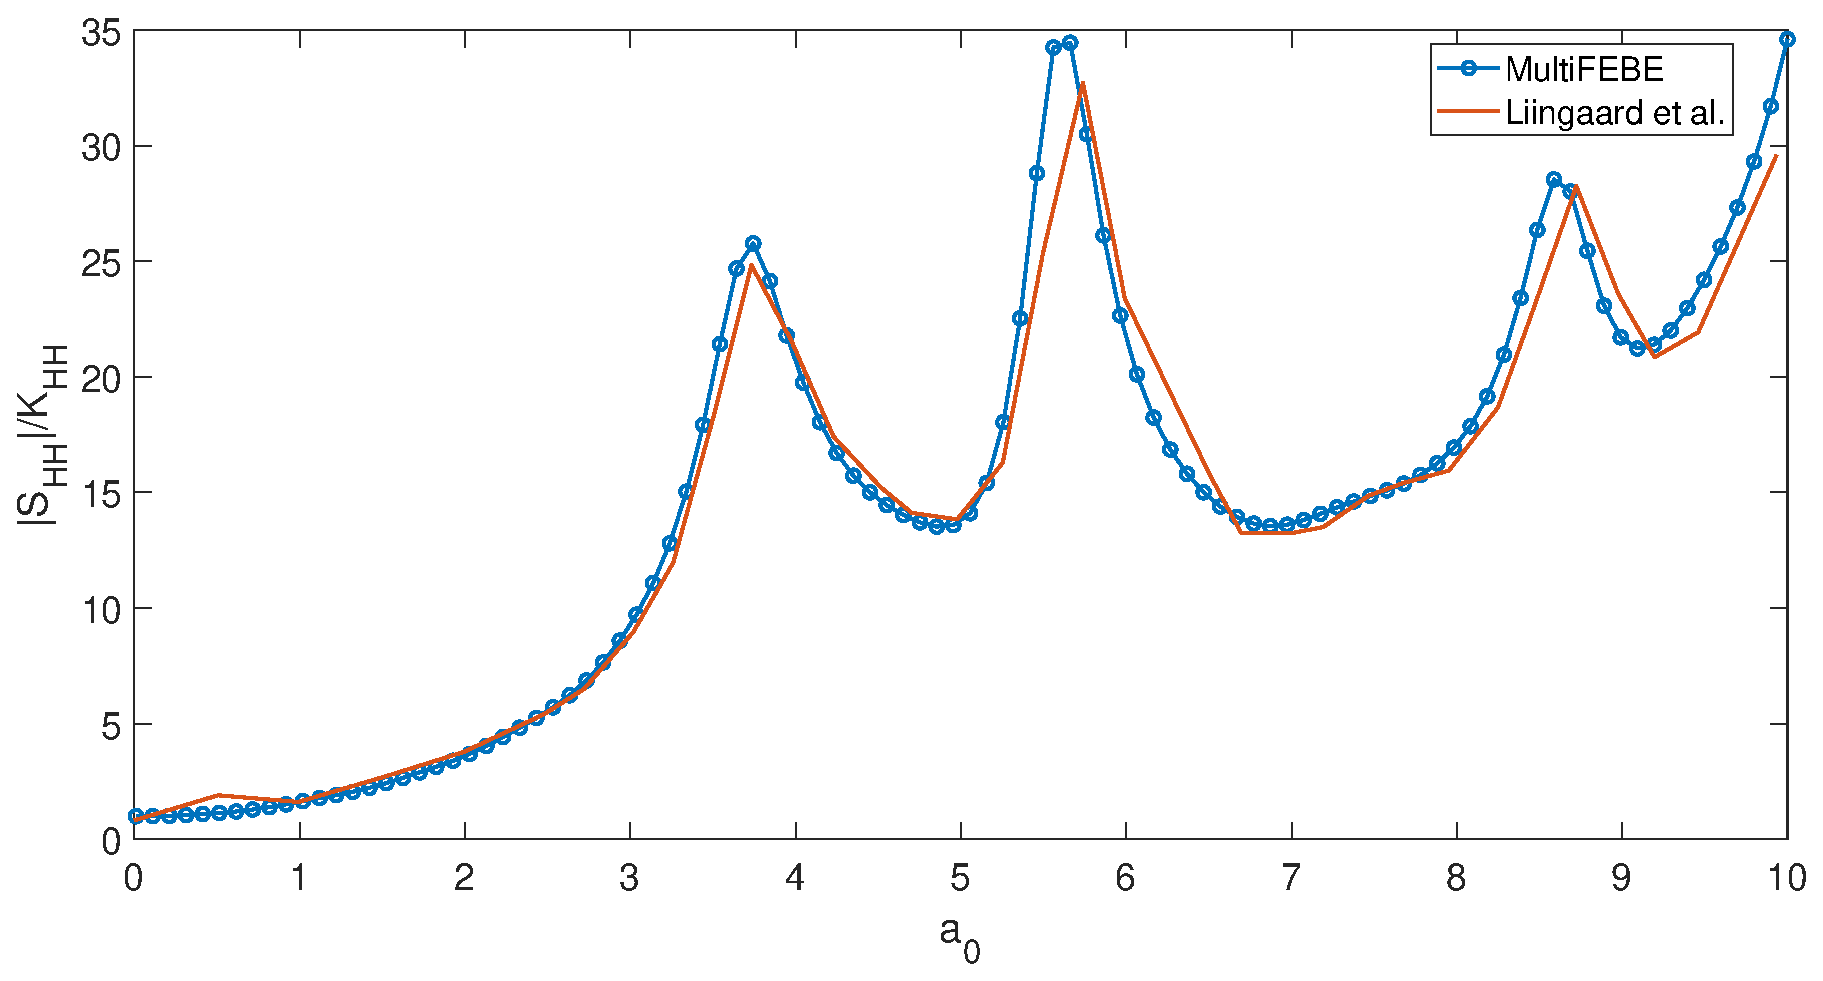
\includegraphics[width=\textwidth]{Shh.eps}
		\label{fig:Shh}
	\end{subfigure}
	\begin{subfigure}[b]{0.48\textwidth}
		\centering
		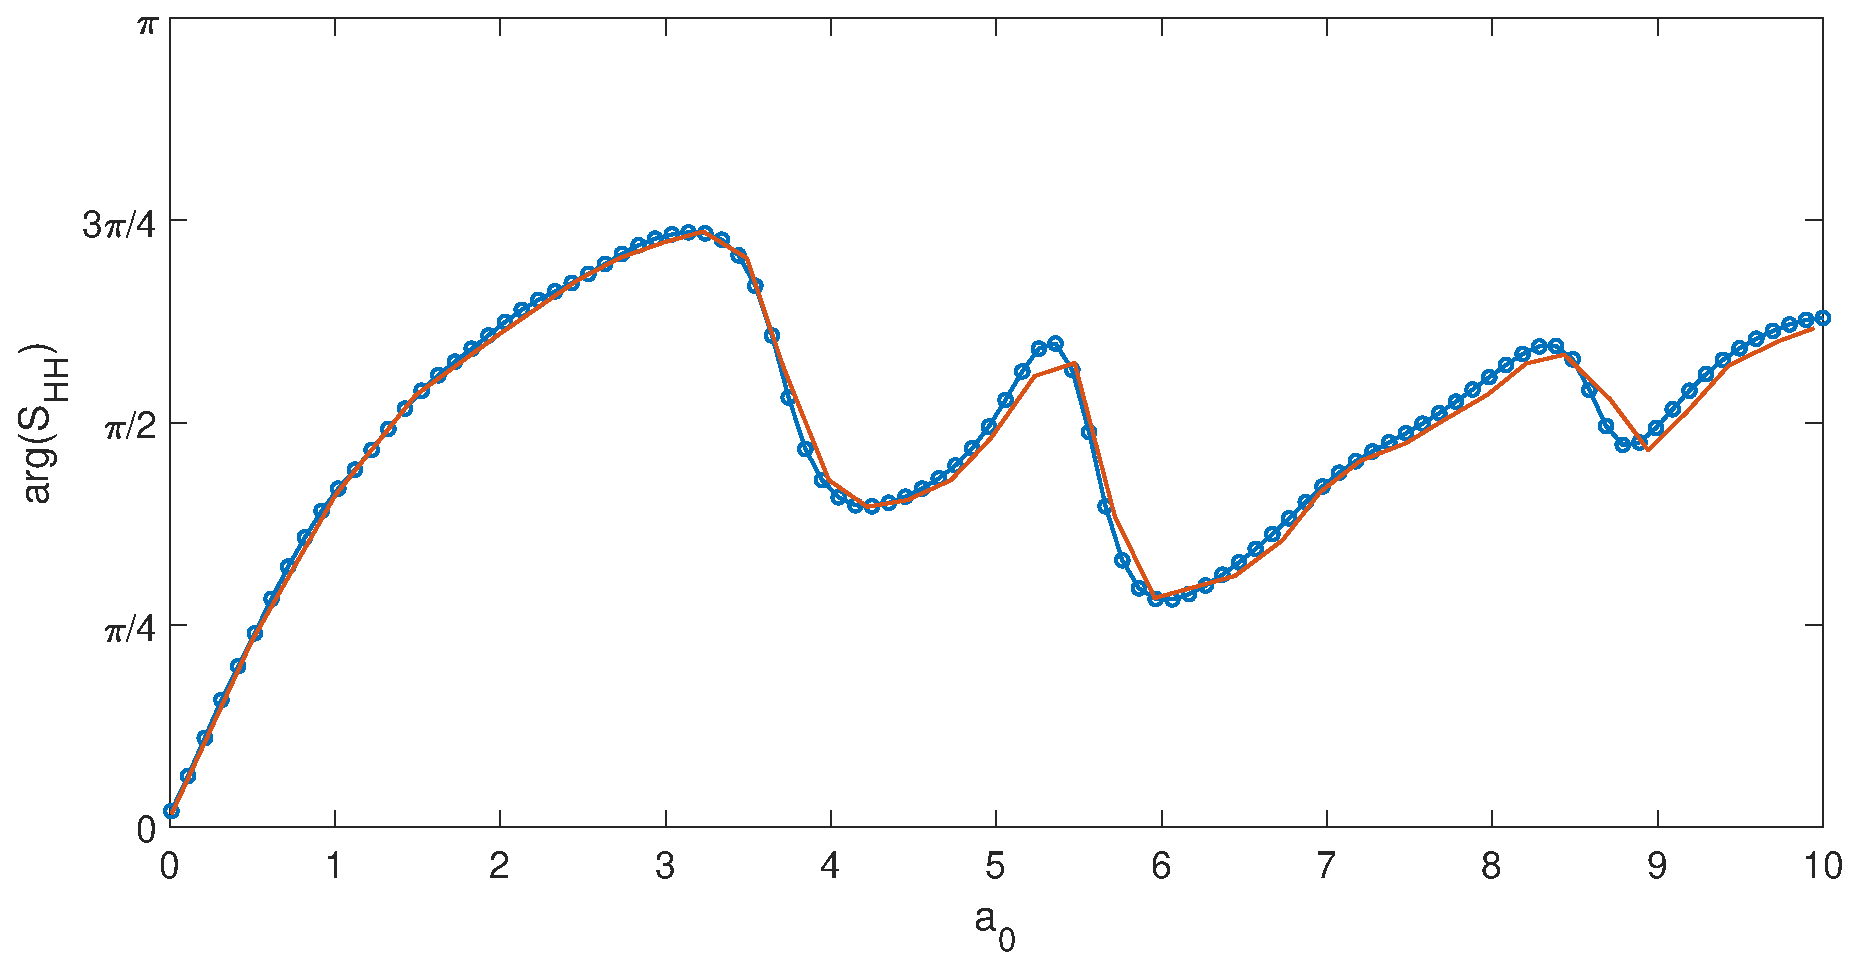
\includegraphics[width=\textwidth]{arg_Shh.eps}
		\label{fig:arg_Shh}
	\end{subfigure}
	\begin{subfigure}[b]{0.48\textwidth}
		\centering
		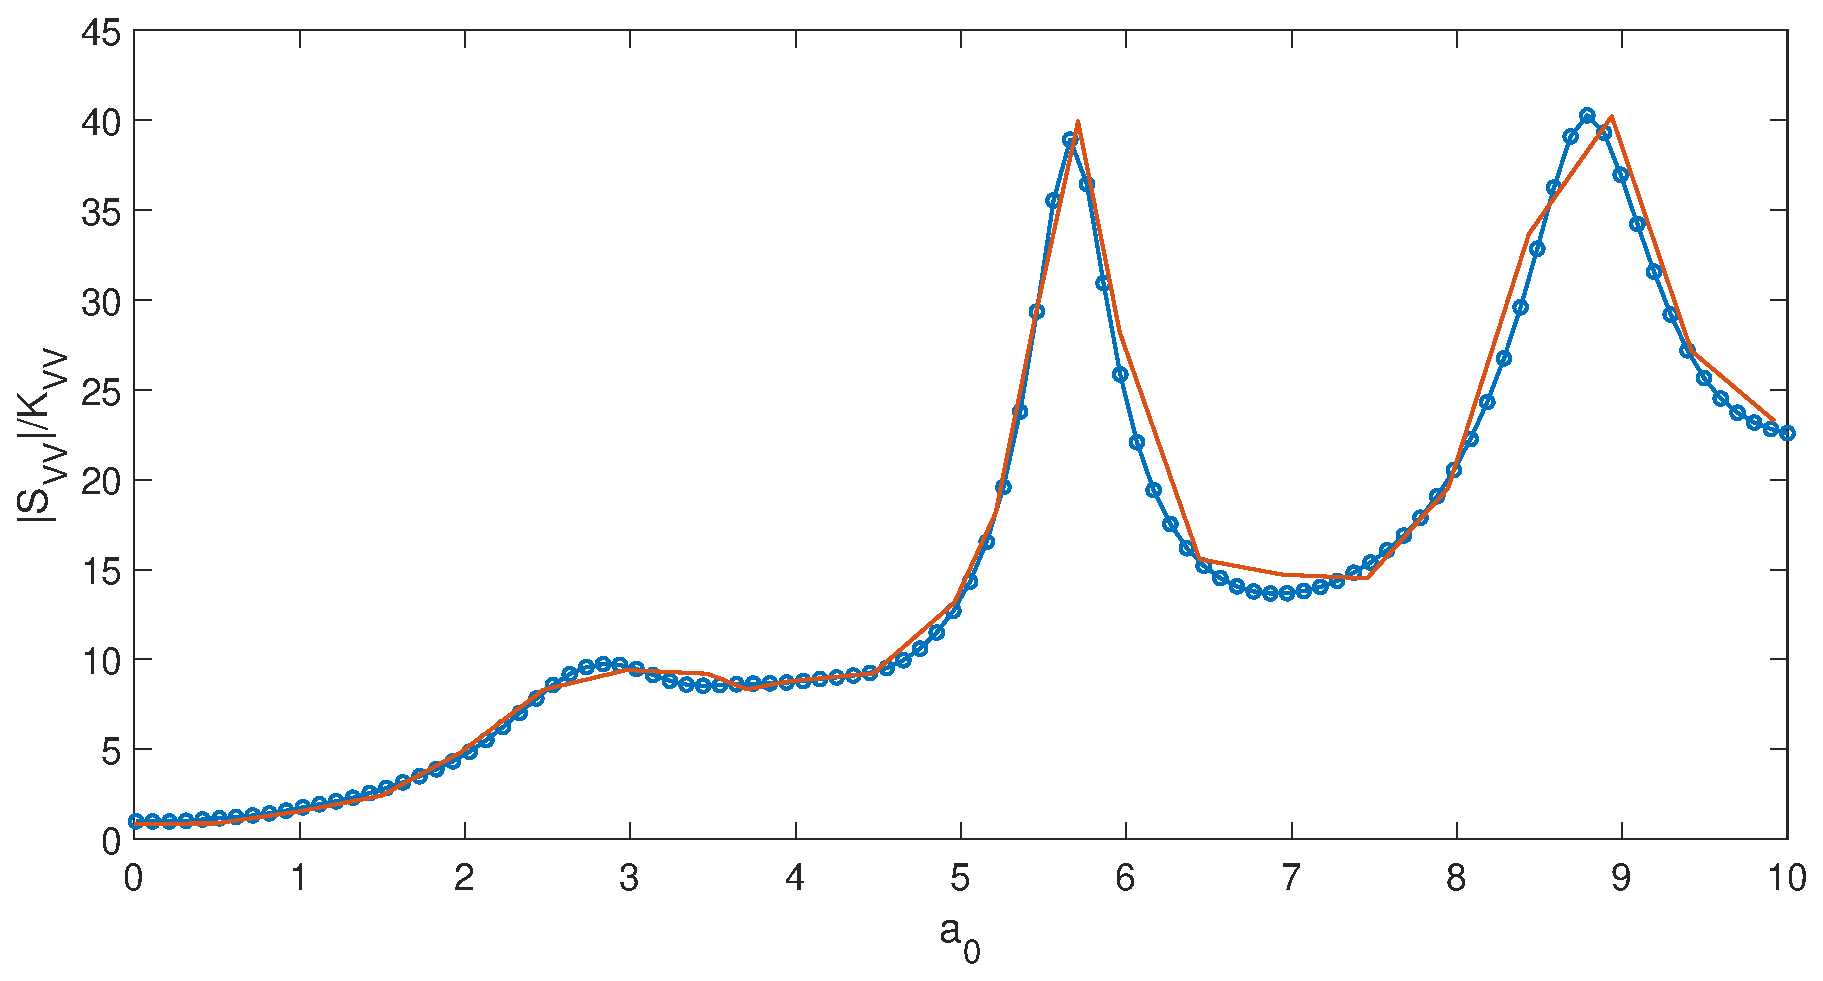
\includegraphics[width=\textwidth]{Svv.eps}
		\label{fig:Svv}
	\end{subfigure}
	\begin{subfigure}[b]{0.48\textwidth}
		\centering
		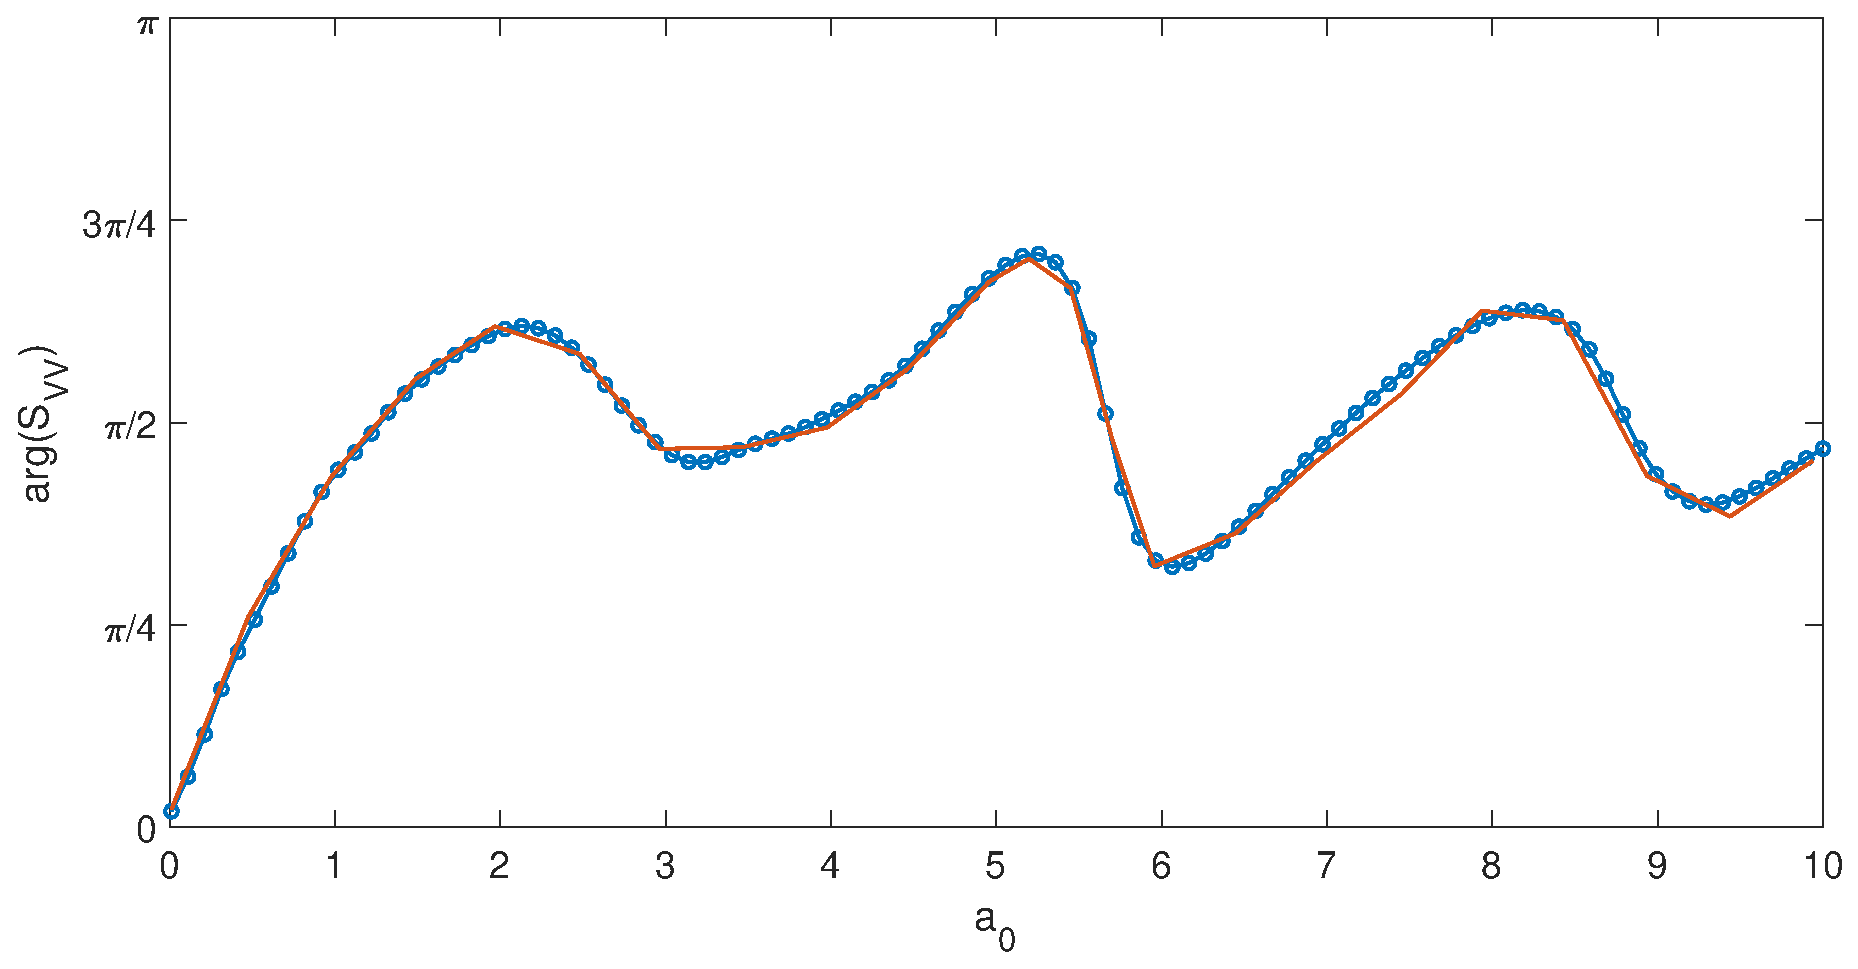
\includegraphics[width=\textwidth]{arg_Svv.eps}
		\label{fig:arg_Svv}
	\end{subfigure}    
		\begin{subfigure}[b]{0.48\textwidth}
		\centering
		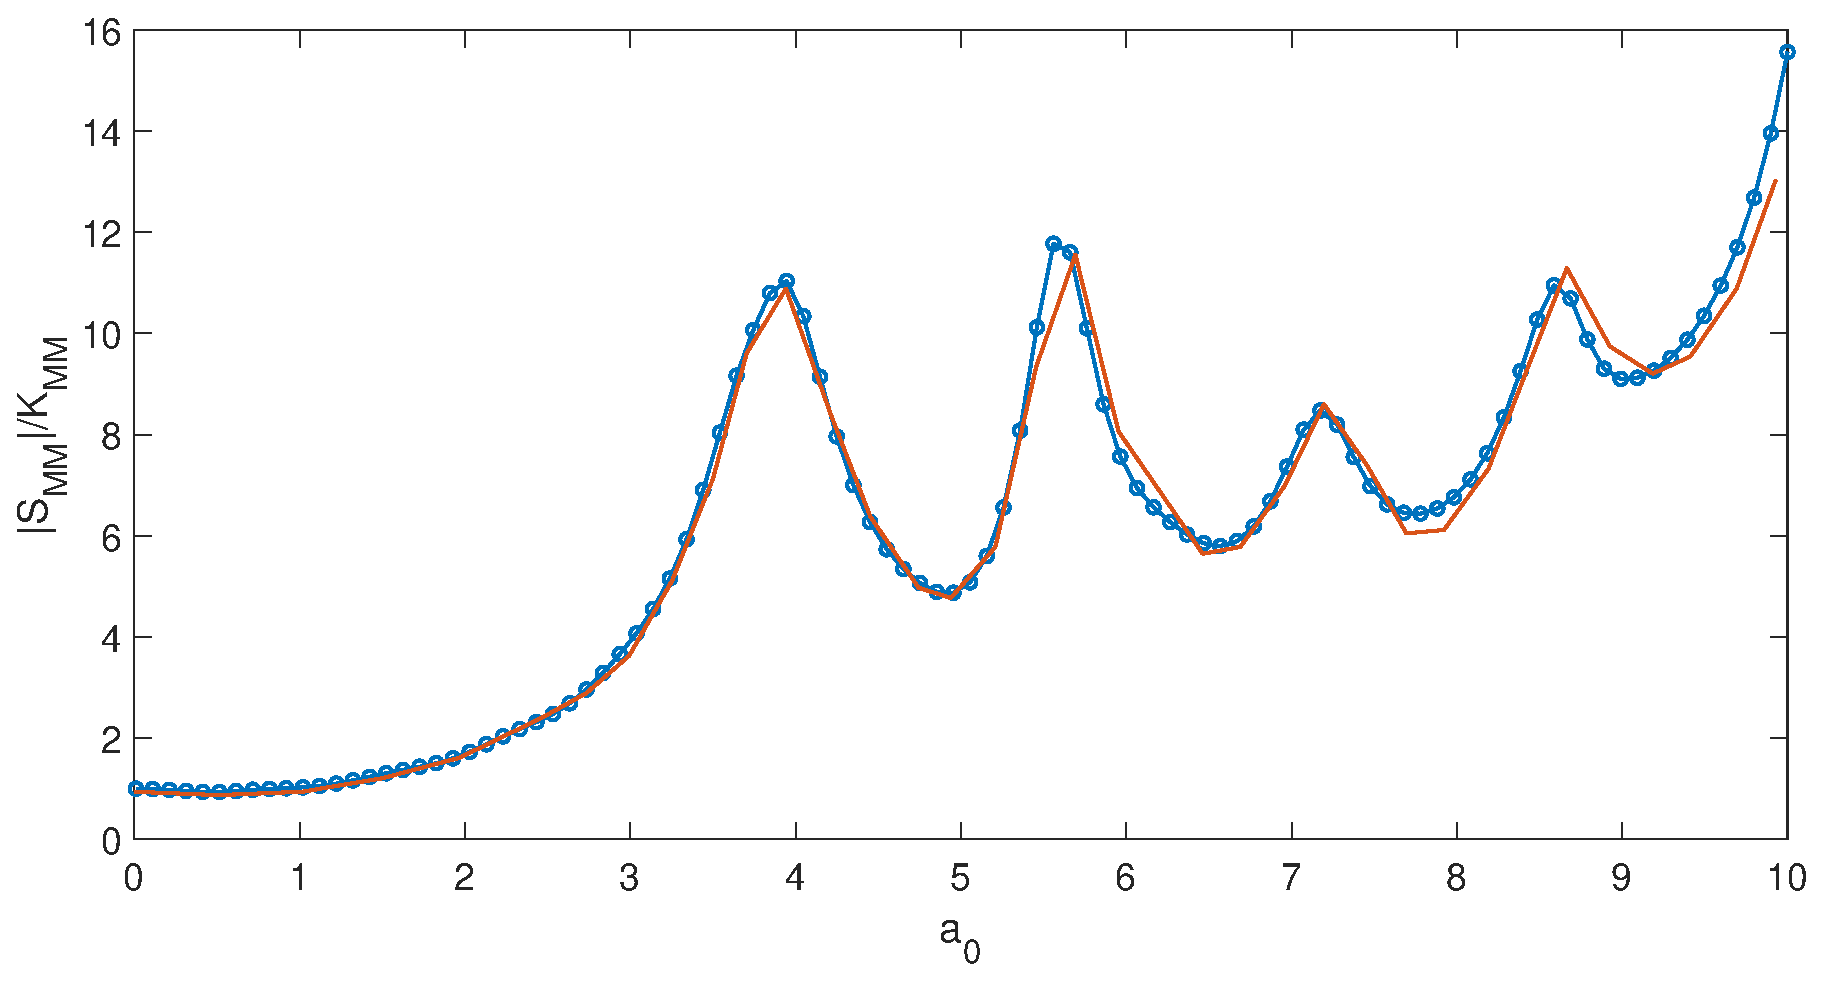
\includegraphics[width=\textwidth]{Smm.eps}
		\label{fig:Smm}
	\end{subfigure}
	\begin{subfigure}[b]{0.48\textwidth}
		\centering
		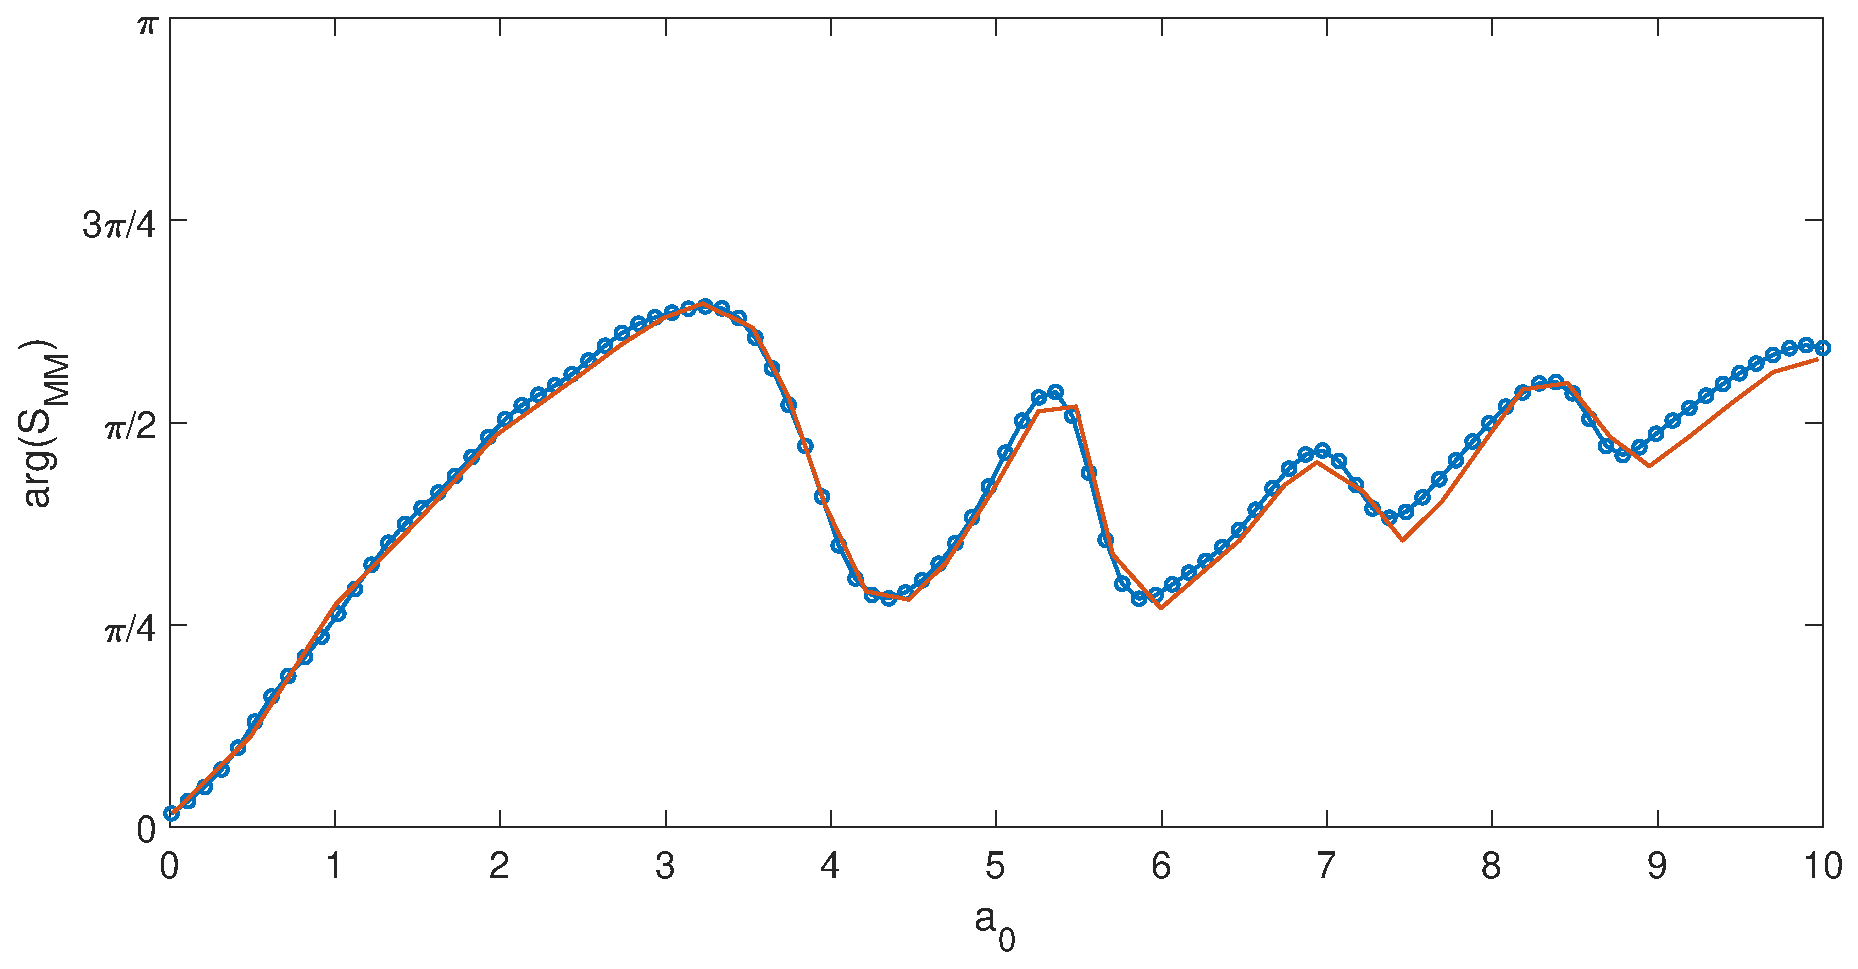
\includegraphics[width=\textwidth]{arg_Smm.eps}
		\label{fig:arg_Smm}
	\end{subfigure}    
	\caption{Normalized horizontal, vertical and rocking impedances. Reference results are taken from \cite{liingaard}.}
	\label{fig:results}
\end{figure}

\FloatBarrier

\begin{thebibliography}{99}
	
<<<<<<< HEAD
	\bibitem{gmsh} C. Geuzaine and J.-F. Remacle, ``Gmsh: a three-dimensional finite element mesh generator with built-in pre- and post-processing facilities." \textit{International Journal for Numerical Methods in Engineering}, Volume 79, Issue 11, pages 1309--1331, (2009).
	
	\bibitem{gmshweb} C. Geuzaine and J.-F. Remacle, ``Gmsh." \url{http://gmsh.info/}
	
	\bibitem{liingaard} M. Liingaard, L. Andersen and L.B. Ibsen, ``Impedance of flexible suction caissons." \textit{Earthquake Engineering and Structural Dynamics}, Volume 36, pages 2249--2271, (2007).
=======
	\bibitem{gmsh} C. Geuzaine and J.-F. Remacle, "Gmsh: a three-dimensional finite element mesh generator with built-in pre- and post-processing facilities." \textit{International Journal for Numerical Methods in Engineering}, Volume 79, Issue 11, pages 1309--1331, (2009).
	
	\bibitem{gmshweb} C. Geuzaine and J.-F. Remacle, "Gmsh." \url{http://gmsh.info/}
	
	\bibitem{liingaard} M. Liingaard, L. Andersen and L.B. Ibsen, "Impedance of flexible suction caissons." \textit{Earthquake Engineering and Structural Dynamics}, Volume 36, pages 2249--2271, (2007).
>>>>>>> main

\end{thebibliography}

\end{document}
